\documentclass[11pt]{article}
\usepackage[margin=0.8in]{geometry}
\usepackage{graphicx,tabularx,booktabs}
\usepackage[colorlinks=true,urlcolor=blue]{hyperref}
\setlength{\parindent}{0pt}\setlength{\parskip}{7pt}\setlength{\emergencystretch}{2em}
\begin{document}
{\LARGE Private-namespace cutoff: mechanism check}\par
{\large One retained software qualification --- 2026-10-30}\par
\textbf{Observed result.} In one isolated fixture container, the unchanged deadline helper stopped a detached child while PID 1's main thread was blocked. The observer recorded the child reaped with signal 9, and the container then exited with code 125. Orchestration and container removal both returned zero. No rerun is included in this report.

\begin{tabularx}{\textwidth}{@{}p{0.35\textwidth}X@{}}\toprule
Observation & Retained value\\\midrule
Fixture admission & PID 1, effective UID 0; child PID 7; monotonic anchor captured.\\
Main thread & Installed marker followed by blocking \texttt{pause}; no deadline polling on the main thread.\\
Detached child & Separate session; observer thread recorded signal 9 and no exit code.\\
Observer elapsed counter & 2,196,991,669 ns from the fixture's initial monotonic timer. Single operational observation, not a benchmark estimate.\\
Container terminal state & Exit 125; not running; OOMKilled false.\\
Start / finish UTC & 22:19:18.805569819 / 22:19:21.103898781.\\
Orchestration / cleanup & Both exit zero; exact owned-container removal recorded.\\\bottomrule
\end{tabularx}

\textbf{Isolation and resource boundary.} Retained inspection specifies a private PID namespace, private IPC, network none, read-only root filesystem, all capabilities dropped, no-new-privileges, no host mounts and no privileged mode. Caps were 64 MiB memory with matching swap limit, 0.25 CPU and 16 PIDs. The fixture required PID 1, effective UID 0 and an explicit qualification marker before calling the source guard. A separate observation thread belongs to PID 1 and survives the namespace-wide child signal.

\textbf{What this checks.} The exact helper's captured deadline path can terminate an owned detached process and a blocked-main supervisor in this inspected private-container configuration. The source uses a 10 ms polling sleep and a 100 ms tail before exit125. This run used ordinary clocks; no clock-adjustment experiment was performed. Production controller/CRIU integration and physical worker deallocation are separate checks.

\newpage
{\Large Evidence, mechanism and review binding}

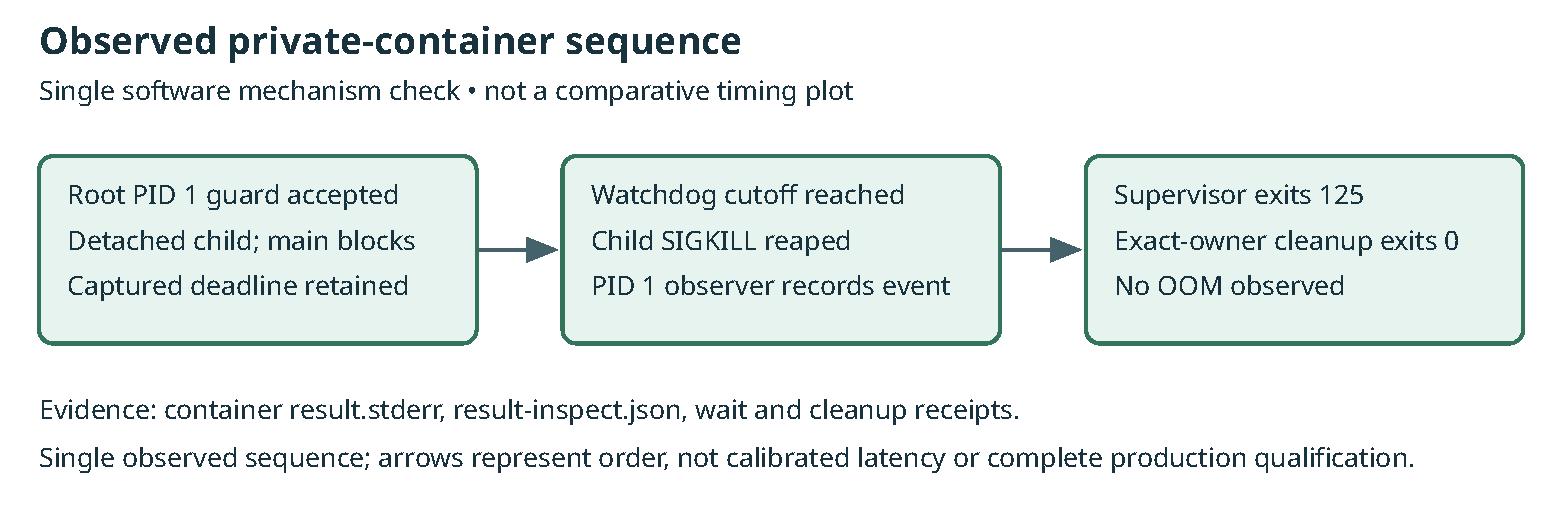
\includegraphics[width=\textwidth]{mechanism.pdf}

\textbf{Exact identities.} The copied unchanged deadline module has SHA-256\\
{\footnotesize\texttt{b7eaf3b0249a7bb630c9a486eb613c48e3ec779c486796c9634c2fdfc61644cb}}.\\
The musl fixture binary has SHA-256\\
{\footnotesize\texttt{7aa53cc278569ca13f1f0d9a860a65de7004b77c854db27f3f56ed819a8dd7f9}}.\\
The local image is identified by\\
{\footnotesize\texttt{sha256:fdee14f586902162cc587d180fa734a9f21e395719e357ac75720345bfeef8df}}.\\
Full container ID, fixture source, lockfile, recipe and v4 orchestration hashes are in the accompanying records.

\textbf{Build and retained failure.} The private offline static build returned zero. The local scratch-image build succeeded. Reading its root-owned image-ID file with unprivileged \texttt{cat} failed; the owner reconciled it with a privileged read rather than rebuilding. This report records that administrative failure separately from the successful image build and mechanism observation. No fixture binary was run on the host.

\textbf{Independent review and additive custody.} Independent review supports one bounded local private-container mechanism observation. Its three original custody gaps are preserved in the review. A later command record supplies the build command, toolchain selection and v4 arguments as an explicitly post-hoc reconstruction, not a contemporaneous signed launch receipt. A new read-only query at 22:22:16 UTC returned zero labelled containers with exit0; it adds a later state observation without rerunning the fixture. The contemporaneous command-provenance limitation remains.


\textbf{Artifact structure.} \texttt{status.json} records observations and scope; \texttt{evidence-manifest.json} binds retained source, configuration, command logs and inspection records. The graph is editable SVG. Raw fixture/runtime binaries are not copied into the report. Original evidence remains unchanged. Report preparation performed no builds, container runs, scientific experiments or runtime publication.
\end{document}
